\documentclass[tikz,border=2pt]{standalone}
\usepackage{amsmath}
\usetikzlibrary{arrows.meta}
\begin{document}
% Pension deferred u = 20 years at age 40: unit payments from time 20 while alive are worth
% ddot a_60 = 12 at time 20; the pure endowment factor {}_20E_40 = 0.3 brings this to 0.3(12) = 3.6 at time 0.
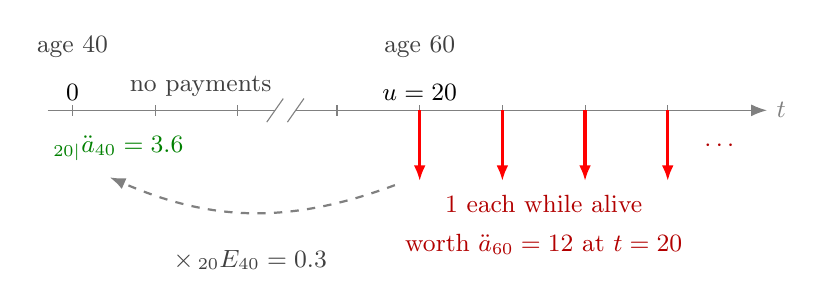
\begin{tikzpicture}[font=\small, >={Latex[length=2mm]}, x=1.05cm, y=1cm]
  % broken time axis: times 0,1,2 | 19,...,23
  \draw[gray] (-0.3,0) -- (2.45,0);
  \draw[gray] (2.35,-0.15) -- (2.55,0.15);
  \draw[gray] (2.6,-0.15) -- (2.8,0.15);
  \draw[gray, ->] (2.7,0) -- (8.4,0) node[right] {$t$};
  \foreach \x in {0,1,2,3.2,4.2,5.2,6.2,7.2} \draw[gray] (\x,-0.07) -- (\x,0.07);
  \node[above, inner sep=2pt] at (0,0.05) {$0$};
  \node[above, inner sep=2pt] at (4.2,0.05) {$u=20$};
  \node[gray!50!black] at (0,0.8) {age $40$};
  \node[gray!50!black] at (4.2,0.8) {age $60$};
  \node[gray!50!black] at (1.55,0.3) {no payments};
  % payments from time u = 20 while alive
  \foreach \x in {4.2,5.2,6.2,7.2} \draw[->, red, very thick] (\x,0) -- (\x,-0.9);
  \node[red!70!black] at (7.85,-0.45) {$\cdots$};
  \node[red!70!black, anchor=north] at (5.7,-0.95) {$1$ each while alive};
  \node[red!70!black, anchor=north] at (5.7,-1.45) {worth $\ddot a_{60}=12$ at $t=20$};
  % back to time 0
  \draw[->, gray, thick, dashed] (3.9,-0.95) to[bend left=22] (0.45,-0.85);
  \node[gray!50!black, anchor=north] at (2.15,-1.65) {$\times\,{}_{20}E_{40}=0.3$};
  \node[green!50!black, anchor=north west] at (-0.35,-0.2) {${}_{20|}\ddot a_{40}=3.6$};
\end{tikzpicture}
\end{document}
